%qqqqqqqqqqqqqqqqqqqqqqqqqqqqqqqqqqqqqqqqqqqqqqqqqqqqqqqqqqqqqqqqqqqqqqqqq
%Quote
%\begin{savequote}[50mm]
%‘‘El cosmos es todo lo que es, todo lo que fue y todo lo que será. Nuestras 
%más ligeras contemplaciones del cosmos nos hacen estremecer: Sentimos como 
%un cosquilleo nos llena los nervios, una voz muda, una ligera sensación como
%de un recuerdo lejano o como si cayéramos desde gran altura. Sabemos que nos
%aproximamos al más grande de los misterios.’’
%\qauthor{Carl Sagan}
%\end{savequote}
%qqqqqqqqqqqqqqqqqqqqqqqqqqqqqqqqqqqqqqqqqqqqqqqqqqqqqqqqqqqqqqqqqqqqqqqqq




%#########################################################################
\chapter{Cosmología y Formación de Estructuras.}
\label{cha:Theoretical Framework}

\section{Relatividad General en el ámbito cosmológico (Universo homogéneo e isótropo )}
\label{sec:IsotropicAndHomogeneousUniverse}
%***********************************************************************
En la naturaleza existen cuatro fuerzas fundamentales. Al considerar un sistema donde interactúan  dos ó más cuerpos con masa, la fuerza que intermedia entre las partículas  es la fuerza de la gravedad. Es por eso que cuando se pretende abordar el estudio de la dinámica de este tipo de interacciones se debe remitir a la teoría de la gravedad. En la actualidad la mejor forma de reproducir la dinámica del universo es haciendo uso de la teoría de la Relatividad de Albert Einstein.
%Cuando se pretende estudiar el funcionamiento del universo en general, se debe invocar la ciencia que se encarga de ello. La cosmología estudia la dinámica del universo, el origen, evolución y futuro del mismo.  %Cuando se introducen la teoría de la relatividad general esta empieza a ser parte de la física, pues las leyes que describen el universo como un todo son las mismas que determinan el funcionamiento de los sistemas que se encuentra adentro de él. Esta teoría se  sustenta por una base matemáticamente robusta que  puede predecir eventos y reproduce las observaciones. 

En el camino de poder estudiar la dinámica del universo, un  paso obligado es conocer las ecuaciones de Einstein y poder ende conocer sus soluciones, que son de gran importancia, porque relaciona la estructura del espacio-tiempo con su contenido de materia y su energía. 
%Estas ecuaciones no pueden dar una solución general exacta, es entonces necesario introducir ....
La cosmología pretende  describir el funcionamiento del universo a muy grandes escalas, donde al despreciar las contribuciones de las galaxias, estrellas y otros objetos es posible obtener solución a las ecuaciones de Einstein.

Aunque la cosmología pueda describir los eventos a grandes escalas es necesario partir de algo, introducir restricciones que permitan reproducir el universo actual. Es por esto, que la cosmología parte de dos principios fundamentales:  

- El primer principio cosmológico, habla sobre la distribución de la materia y la forma del universo a medida que evoluciona. Si se toma un punto cualesquiera en el espacio, la distribución  alrededor de él es invariante en el tiempo, sin importar la dirección en la cual se observe. Una forma más estricta de decir este principio es:\\

{\bf{Principio cosmológico:}} {\textit{El cualquier momento, el universo es homogéneo e isótropo a muy grandes escalas.}} (Bert Janssen,2013,p. 207). \\

Cuando se cuenta con un espacio el cuál es homogéneo e isótropo este espacio presenta un máximo de simetría.  Matemáticamente, nos dice que la métrica es invariante bajo cualquier rotación o traslación. 

?`Qué tan cierto puede llegar a ser esto? ?` el universo sí es homogéneo e isótropo ? Cuando se observa el universo, la materia tiende a estar concentrada, las estrellas se concentran en galaxias, las galaxias en cúmulos de galaxias y a su vez estos cúmulos en otros súper cúmulos. Entonces, ?`que tan cierto es que el universo sea homogéneo? Para tener un universo homogéneo e isótropo se debe considerar observaciones a una escala mucho mayor (en el orden de $10^{9}$ años luz), un ejemplo es la radiación cósmica de fondo, que corresponde a la radiación térmica proveniente del origen del universo, la cual tiene una anisotropía del orden de $\Delta T /T \approx= 10^{-5}$. 

- El segundo principio cosmológico trata sobre la dinámica de las sobre densidades en el universo, el cual enuncia que el  movimiento es despreciables cuando se compara con el movimiento cosmológico. El segundo principio se denomina como Postulado de Weyl el cual dice: \\

{\bf{Postulado de Weyl:}} {\textit{La materia a escalas cosmológicas se comporta como un fluido perfecto, cuyas componentes se mueven a lo largo de geodésicas temporales, que no se intersectan, salvo (posiblemente) en un punto en el pasado.}} (Bert Janssen,2013,p. 209)\\

El postulado de Weyl implica una idea muy importante en la cosmología, los observadores privilegiados. Estos observadores  se encuentran en reposo con respecto al fluido, lo cual implica que su movimiento es con respecto a la evolución del universo. El nombre que se le dan a estos observadores son los observadores comóviles. Cuando se define este tipo de observadores también se define un tiempo cosmológico, que corresponde a la dirección temporal del observador comóvil. 



%*************************************************************************
%Geometría
\section{Geometría}
\label{sec:Geometría}
%***********************************************************************

%---------------------------------------------------------------------
	%Metrica
	\subsection{Métrica}
	\label{subsec:Metrica}
	%---------------------------------------------------------------------
	
En la relatividad general la métrica permite definir distancias, ángulos y volúmenes en un espacio Euclideo. Además juega un papel importante porque convierte las coordenadas dependientes del observador $X^{\mu}=(t,x^{i})$ en elementos de línea invariante


\begin{equation}
ds^{2}=\sum_{\mu,\nu}^{4} g_{\mu\nu}dX^{\mu}dX^{\nu} \equiv g_{\mu\nu}dX^{\mu}dX^{\nu} \,.
\label{eq:tensor_metrico}
\end{equation}

La métrica tiene una dependencia espacial y temporal $g_{\mu\nu}(t,{\bf{x}})$, entonces dependerá de donde se esté tomando y en que momento. Por esta dependencia espacio-temporal la métrica también dependerá de la distribución de la materia y la energía, debido a que esta debe reproducir los efectos de la gravedad.

La elección de la métrica responde al universo que se quiere. Para un universo homogéneo e isótropo se puede considerar un sistema con simetría esférica. La expresión para describir el diferencial de longitud entre dos puntos sobre la superficie de una esfera se escribe de la forma

\begin{equation}
dl^{2}=R_{c}^{2}d\theta^{2}+R_{c}^{2}\sin^{2}\theta d\phi^{2} \,,
\label{metrica_esfera}
\end{equation}
%
donde $R_{c}$ es el radio de curvatura de la esfera. La figura (\ref{fig:diferencial_linea_esferico}) presenta el diferencial de línea para una simetría esférica.


%------------------------------------------------------
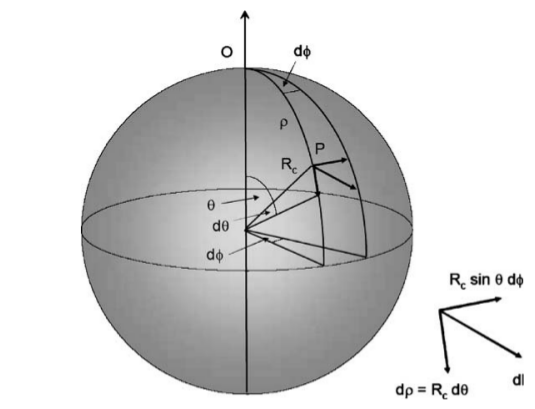
\includegraphics[scale=.4]{./figures/2_theoretical_framework/diferencial_linea.png}
\figcaption{\emph{Representación del diferencial de línea para simetría esférica.}}\label{fig:diferencial_linea_esferico}


%------------------------------------------------------

Usando la figura (\ref{fig:diferencial_linea_esferico}) se construye un arco $\rho$ entre los puntos O y P cuya distancia es $\rho=\theta R_{c}$, entonces la ecuación (\ref{metrica_esfera}) puede reescribirse de la forma

\begin{equation}
dl^{2}=d\rho^{2}+R_{c}^{2}\sin^{2}\left(\frac{\rho}{R_{c}} \right)d\phi^{2} \,.
\end{equation}
%
Una forma alternativa de escribir la métrica es introduciendo una distancia

\begin{equation}
x=R_{c}\sin\left(\frac{\rho}{R_{c}} \right) \,.
\end{equation}
%
Al calcular el diferencial y elevando al cuadrado se obtiene
%
\begin{equation}
dx^{2}=\left[1-\sin^{2}\left( \frac{\rho}{R_{c}}\right) \right]d\rho^{2}  \,, \hspace{1cm} d\rho^{2}=\frac{d^{2}}{1-kx^{2}} \,,
\end{equation}
%
donde $k=1/R_{c}^{2}$ es el parámetro de curvatura.

Por lo tanto la métrica se puede escribir de la forma 

\begin{equation}
dl^{2}=\frac{dx^{2}}{1-kx^{2}}+x^{2}d\phi^{2} \,.
\end{equation}

Se debe recordar que la constante de curvatura $k$ puede representar tres tipos de geometrías: Cuando se tiene una curvatura positiva se obtiene simetría esférica cerrada, con curvatura cero se obtiene el espacio Euclideo plano y si es negativo se tiene una geometría hiperbólica abierta. Ver figura (\ref{fig:curvatura_k}).\\

%-----------------------------------------
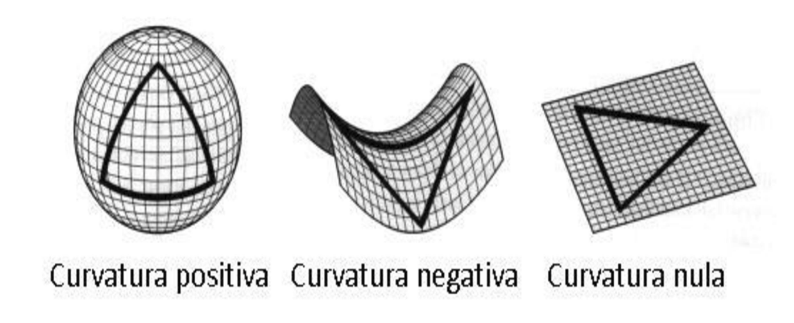
\includegraphics[scale=.4]{./figures/2_theoretical_framework/curvatura_k.png}
\figcaption{\emph{Tres espacios con curvatura constante, esfera con curvatura positiva (izquierda), hiperboloide con curvatura negativa (centro) y plano con curvatura cero (derecha)}.}\label{fig:curvatura_k}

%--------------------------------------------

Extrapolando el diferencial de linea a tres dimensiones en termino de las coordenadas polar esférica $(\rho, \theta, \phi)$ se llega a 

\begin{equation}
dl^{2}=d\rho^{2}+R^{2}_{c}\sin^{2}\left(\frac{\rho}{R_{c}}\right)[d\theta^{2}+\sin^{2}\theta d\phi]\,,
\end{equation}
%
y como se hizo anteriormente también se puede llegar a la ecuación en termino de $x, \theta, \phi$

\begin{equation}
dl^{2}=\frac{x^{2}}{1-kx^{2}}+ x^{2}[d\theta^{2}+\sin^{2}\theta d\phi]\,.
\end{equation}
%
Ahora se puede dar el salto de escribir la métrica considerando el tiempo y llegar a una métrica espacio-temporal

\begin{equation}
ds^{2}=dt^{2}-\frac{1}{c^{2}}dl^{2}\,.
\label{ec:metrica_general}
\end{equation}

Para un modelo isotrópico, se tiene una función que permite describir como cambia la distancia entre dos observadores cualesquiera en un instante de tiempo. $a(t)$ es conocido como el factor de escala y viene dada por 

\begin{equation}
\rho(t)=a(t)r\,,
\end{equation} 
%
r es llamada la \textit{ coordenada radial de distancia comóvil}. Se establece que $a(t)=1$ si $t=t_{o}$ que equivale al universo de hoy.\\

Llamando $R_{c}(t_o)$ como el radio de curvatura para la presente época entonces, $\Re$ se relaciona de la forma

\begin{equation}
R_{c}=a(t)\Re \,.
\end{equation}
%
Sustituyendo $\rho$ y $R_{c}$ en la métrica (\ref{ec:metrica_general}) y considerando $d\Omega^{2}=d\theta^{2}+\sin^{2}\theta d\phi^{2}$ se obtiene 

\begin{equation}
ds^{2}=dt^{2}-\frac{a^{2}(t)}{c^{2}}[dr^{2}+\Re^{2}\sin^{2}(r/\Re)d\Omega^{2}]\,.
\end{equation}
%
Esta es la métrica de Robertson-Walker. Es importante notar que $a(t)$ describe la dinámica del universo y $\Re$ describe la curvatura espacial del universo en la presente época.

Otra forma de representar la métrica es usando \textit{diametro angular comóvil} $r_{1}=\Re\sin(r/\Re)$

\begin{equation}
ds^{2}=dt^{2}-\frac{a^{2}(t)}{c^{2}}\left[\frac{dr^{2}_{1}}{1-kr^{2}_{1}}+r^{2}_{1}d\Omega^{2}\right]\,,
\end{equation}
%
donde $k=1/\Re^{2}$.

Retomando la ecuación inicial (\ref{eq:tensor_metrico}), el tensor métrico $g_{\mu\nu}$ sería


%\begin{bmatrix}
%1 & 0 & 0 & 0\\ 
%0 & $\frac{-a^{2}(t)}{1-kr^{2}}}$ & 0  & 0\\ 
%0 & 0 & $-a^{2}(t)^{2} $  & 0 \\ 
%0 & 0 & 0 & $-a^{2}(t)\sin^{2}(\theta)$
%\end{bmatrix}


\begin{equation}
g_{\mu\nu}=
\begin{bmatrix}
1 & 0 & 0 & 0 \\ 
0 & \frac{-a^{2}(t)}{1-kr^{2}} & 0 & 0 \\ 
0 & 0 & -a^{2}(t)  & 0 \\ 
0 & 0 & 0 & -a^{2}(t)\sin^{2}(\theta)
\end{bmatrix}\,.
\end{equation}


%\newpage
%*************************************************************************
%The Friedmann equations
\section{Ecuaciones de Friedmann}
\label{sec:Ecuaciones_Friedmann}
%************************************************************************

En Relatividad General, las ecuaciones de campo de Einstein brindan información muy importante sobre la relación entre la energía, masa y la geometría del espacio-tiempo, cuya relación es dada por 

\begin{equation}
R_{\mu\nu}-\frac{1}{2}R-g_{\mu\nu}\Lambda=\frac{8\pi G}{c^{4}}T_{\mu\nu} \,,
\label{eq:Einstein_campo_ecuacion}
\end{equation}
%
donde $R_{\mu\nu}$ es el tensor de Ricci, $R$ es el escalar de Ricci, $g_{\mu\nu}$ es la métrica, $\Lambda$ constante cosmológica y $T_{\mu\nu}$ es el tensor momentum-energía. 

El tensor y escalar de Ricci se pueden calcular de la siguiente manera

\begin{eqnarray}
R_{\mu\nu} \equiv \partial_{\lambda}\Gamma^{\lambda}_{\mu\nu} - \partial_{\nu}\Gamma^{\lambda}_{\mu\lambda} + \Gamma^{\lambda}_{\lambda\rho} \Gamma^{\rho}_{\mu\nu} - \Gamma^{\rho}_{\mu\lambda} \Gamma^{\lambda}_{\nu\rho}\,,
\end{eqnarray}

\begin{equation}
R=R^{\mu}\,_{\mu}=g^{\mu\nu}R_{\mu\nu}\,,
\label{eq:Tensor_Ricci}
\end{equation}
%
donde 

\begin{equation}
\Gamma^{\nu} \,_{\alpha\beta}=\frac{1}{2}g^{\mu\sigma}(\partial_{\beta} g_{\sigma\alpha}+\partial_{\alpha} g_{\sigma\beta}-\partial_{\sigma} g_{\alpha\beta})\,.
\end{equation}

Debido a la isotropía del espacio en la métrica de \textit{Robertson-Walker}, no es necesario calcular las componentes $R_{i0}=R_{oi}$. Las componentes que no se hacen cero del tensor de Ricci son


\begin{eqnarray}
R_{00}=-3\frac{\ddot{a}}{a}\,, \hspace{2cm} \\
R_{ij}=-\left[\frac{\ddot{a}}{a}+ 2\left(\frac{\dot{a}}{a}\right)^{2} + 2\frac{k}{a^{2}} \right]g_{ij} \hspace{1cm} i,j=0,1,2\,,
\end{eqnarray}

\begin{align}
R_{\mu\nu}=R_{00}+R_{ij}\,,
\label{eq: tensor_Ricci}
\end{align}

y el escalar de Ricci queda 

\begin{equation}
R=-6\left[\frac{\ddot{a}}{a} + \left(\frac{\dot{a}}{a} \right) + \frac{k}{a^{2}} \right]\,.
\label{eq:Ricci_escalar}
\end{equation}

En cosmología cuando se pretende calcular el tensor momentum-energía, se considera  un fluido perfecto. Tomando el tensor como la suma de sus componentes $T_{\mu\nu}=T_{ij}+T_{i0}+T_{0j}+T_{00}$, y debido a la isotropía se tiene que $T_{i0}=T_{0j}=0$. Al considerar entonces la isotropía y la homogeneidad se tiene

\begin{equation}
T_{00}= \rho(t)\,, \hspace{1cm} T_{io}=0\,, \hspace{1cm} T_{ij}=-P(t)g_{ij}(t,\bf{x})\,.
\label{eq: Tensor_momentum-energia}
\end{equation}
%
Remplazando (\ref{eq: Tensor_momentum-energia}), (\ref{eq:Ricci_escalar}) y (\ref{eq: tensor_Ricci}) en la ecuación (\ref{eq:Einstein_campo_ecuacion}), se permiten llegar a dos ecuaciones escalares acopladas

\begin{equation}
\frac{\ddot{a}}{a} = -\frac{4\pi G}{3}\left(\rho + \frac{3P}{c^{2}} \right) + \frac{c^{2}\Lambda}{3}\,,
\end{equation}
\begin{equation}
\frac{\ddot{a}}{a}+2 \left(\frac{\dot{a}}{a}\right)^{2} + 2k\left(\frac{c}{a} \right)^{2} =4\pi G\left( \rho - \frac{P}{c^{2}}\right)+ c^{2}\Lambda\,,
\end{equation}
%
donde $\rho$ es la densidad y $P$ es la presión.

La importancia de estas ecuaciones radica en que permiten conocer la evolución del universo (homogéneo e isótropo) usando el factor de escala. 


%*************************************************************************
%The Friedmann equations
\section{Formación de Estructuras.}
\label{sec:Estructure_Formation}
%************************************************************************



%Buscando poder demostrar un modelo que permita modelar la estructura del universo a gran escala, se hace uso de la {\it{Inestabilidad de Jeans}}. Esta teoría representa la evolución del universo, partiendo de los principios fundamentales (homogeneidad e isotrpía).

Al observar el universo a gran escala, es claro que posee alta simetría y homogeneidad, pero ?`qué pasa cuando se mira a escalas menores? A escalas menores que la cosmológicas, los sistemas son asimétricos e inhomogéneos, lo cual implica una alta complejidad. Por esto, es necesario realizar modelos que permitan reproducir lo observacional, asumiendo aproximaciones coherentes,  haciendo que el grado de dificultad disminuya. El universo a escalas menores que las cosmológicas, presenta no linealidad en casi todos sus sucesos; la formación de estructuras es un caso de ello. La forma de introducir la linealidad o no linealidad en la formación de estructuras es considerando el campo de densidad. Para él régimen lineal se supone ($\delta\rho << \bar{\rho}$), donde la perturbación de la densidad es mucho menor que la densidad media. Mientras que para el régimen no lineal se supone que la perturbación es aproximada a la densidad media ($\delta\rho \sim \bar{\rho}$).


Con el propósito de poder reconstruir la estructura del universo en cualquier instante $t$ se considera lo siguiente:

Al observar el pasado, se debe pensar que existieron pequeñas desviaciones en la homogeneidad en la materia. A medida que el tiempo pasa, estas desviaciones incrementan, debido a la fuerza gravitacional. Esto fue generando una acumulación de materia cada vez mayor, que desencadeno la formación de estructuras, y que dieron origen a las primeras galaxias. Las soluciones a las ecuaciones de Friedmann permiten incrustar las perturbaciones que dan origen a la formación de estructuras.

Se debe tener presente que la teoría del régimen lineal solo se cumple para desviaciones pequeñas, osea, para un universo muy joven. Para poder reproducir las estructuras del universo observable, es necesario considerar un teoría de régimen no lineal. 


%*************************************************************************
%The Friedmann equations
\subsection{Régimen Lineal Para la Formación de Estructuras.}
\label{subsec:Lineal_Estructure_Formation}
%************************************************************************


%---------------------------------------------------------------------
	%M
	\subsubsection{Régimen Newtoniano.}
	\label{subsubsec:Newtonian_Regimen}
	%---------------------------------------------------------------------


En el régimen lineal la perturbación en la métrica $g_{\mu\nu}$ y su fuente $T_{\mu\nu}$ se escriben de la forma

\begin{equation}
g_{\mu\nu} \Rightarrow g_{\mu\nu}+\delta g_{\mu\nu} \hspace{0.8cm} T_{\mu\nu} \Rightarrow T_{\mu\nu} +\delta T_{\mu\nu} \,.
\end{equation}
%
Al supone que las perturbaciones son pequeñas es posible linealizar la ecuación de Einstein 

\begin{equation}
\hat{\mathcal{L}}(g_{\mu\nu})\delta g_{\mu\nu} = \delta T_{\mu\nu} \,,
\end{equation}
%
donde $\hat{\mathcal{L}}$ es el operador diferencial lineal que depende del espacio-tiempo. 
 
Una forma simple de poder calcular la dinámica de las perturbaciones es infiriendo que el radio de la perturbación es menor al radio de Hubble. Al decir esto se puede obviar del caso relativista y considerarlo meramente Newtoniano. Al suponer esto, se puede considerar la materia del universo como un fluido Newtoniano que colisiona. Esto implica que es posible usar las ecuaciones de un fluido Newtoniano:

\begin{eqnarray}
\frac{\partial \rho}{\partial t} + \nabla\cdotp(\rho v) = 0\,, \hspace{1cm} Ecuacion\ de\ continuidad \\
\label{eq: Navier-Stoke1}
\frac{\partial v}{\partial t} +(v\cdot \nabla)v = -\frac{\nabla p}{\rho}- \nabla\Phi \,,  \hspace{0.5cm} Ecuacion\ de\ Euler\\
\label{eq: Navier-Stoke2}
\nabla^{2}\Phi = 4\pi G\rho\,. \hspace{1.3cm} Ecuacion\ de\ Poisson\\
\label{eq: Navier-Stoke3}
\end{eqnarray}

Al aplicar las pequeñas perturbaciones cuasiestáticas a la densidad ($\rho=\rho_{o}+\delta\rho$), velocidad ($v=\delta v$), presión ($p=p_{o}+\delta p$) y al potencial gravitacional ($\Phi=\Phi_{o}+\delta\Phi$). Se obtiene 

%\begin{subequations}
\begin{align}
\frac{\partial \delta\rho}{\partial t} + \rho_{o}\nabla\cdotp(\delta v) = 0\,,
\label{eq:Navier-stoke1_perturbation}
\end{align}
%----------------
\begin{align}
\frac{\partial \delta v}{\partial t} + \frac{1}{\rho}\left(\frac{\partial p}{\partial \rho} \right)\nabla \delta \rho+ \nabla\delta\Phi =0\,,
\label{eq:Navier-stoke2_perturbation}
\end{align}
%-------
\begin{align}
\nabla^{2}\delta\Phi - 4\pi G\delta\rho = 0\,.
\label{eq:Navier-stoke3_perturbation}
\end{align}	
%\end{subequations}

Ahora el propósito es poder resolver las ecuaciones con perturbaciones (\ref{eq:Navier-stoke1_perturbation}, \ref{eq:Navier-stoke2_perturbation}, \ref{eq:Navier-stoke3_perturbation}). Para ello  se puede suponer soluciones de ondas planas\footnote{Cuando se supone un universo plano, se consideró la aparición de las ondas planas}

\begin{equation}
\delta u_{i} = \delta_{i}e^{i\bf{k}\cdot \bf{r}}\,,
\end{equation}
%
donde $\delta u_{i}= \delta\rho, \delta v, \delta\Phi$ y se entiende que $\delta_{i}$ equivale a las amplitudes. Permitiendo facilidad en los cálculos. 
%%Mi propósito no es solucionar estas ecuaciones, solo pretendo mostrar que consideraciones se deben hacer para llegar a los resultados
~\\
Al considerar la inestabilidad gravitacional, se puede obtener unos resultados  interesantes sobre la formación de la estructura. Entonces considerando lo siguiente: 

Para un fluido homogéneo e isotrópico, Jeans dice que a medida que el sistema va evoluciona se van generando pequeños cambios en la densidad $\delta \rho$ y en la velocidad $\delta v$.

De igual manera Jeans plantea que la aparición de una inhomogeneidad en la distribución de materia $\delta\rho$  generará un cambio en la fuerzas que preservan la homogeneidad. Entonces si $\delta\rho>0 $  la fuerza de gravitación $F_{g}$(responsable del colapso) deberá ser mayor que la fuerza de presión $F_{p}$(responsable del no colapso), entonces   $F_{g}>F_{p}$. Esta ultima afirmación da la condición necesaria para la formación de estructuras. Usando esta idea se puede determinar el radio necesario para el cuál se cumple la desigualdad, también conocido como el radio de Jeans $\lambda$.  

\begin{eqnarray}
F_{g} \approx G\rho\lambda \ \ \  y \ \ \ F_{p}\approx\frac{v_{s}^{2}}{\lambda}\\
\lambda^{2} > \frac{v_{s}^{2}}{G\rho} \,,
\end{eqnarray}

de una forma similar se puede llegar al tiempo gravitacional de caída libre 

\begin{equation}
\tau_{f-f} \approx \frac{1}{(G\rho)^{1/2}}\,.
\end{equation}


%*************************************************************************
%The Friedmann equations
\subsection{Régimen no lineal Para la Formación de Estructuras.}
\label{subsec:non-Lineal_Estructure_Formation}
%************************************************************************

Cuando se observo el universo en sus etapas tempranas, antes de la era de la recombinación\footnote{Instante en el universo donde la temperatura bajo lo suficiente para poder permitir la combinación de los electrones con los nucleos generando los primeros átomos. Antes de este instante se conoce como la época dominada por la radiación, electrones y protones libres.}, se consideró que las fluctuaciones $\delta$  en la materia eran despreciables ($\delta \ll 1$). Esta suposición permite facilitar muchos cálculos, pero restringe el tiempo de evolución del universo. Sin embargo, si se pretende determinar la evolución y estructuras a escalas mayores como en la actualidad, donde $\delta \gg 1$, es necesario hacer uso de otro método que permita reconstruir la dinámica del universo. Para ello se hace uso del régimen no lineal. Cabe resaltar que esta técnica es altamente complicada donde es necesario hacer aproximaciones y muchas veces no es posible llegar a soluciones analíticas, por esto se hace uso de los métodos numéricos que permiten encontrar aproximaciones a las soluciones. 

En la actualidad existe una gran variedad de métodos que describen la formación no lineal. Un caso especial es la aproximación de Zeldovich, la cual es capaz de reproducir el régimen lineal, permitiendo usar una  expresión analítica y reduciendo la complejidad de los cálculos. Este método además reproduce de muy buena manera el universo observable actual.

%-----------------------------------------
%\includegraphics[scale=.4]{./figures/2_theoretical_framework/Zeldovich.gif}
%\figcaption{\emph{Tres espacios con curvatura constante, esfera con curvatura positiva (izquierda), hiperboloide con curvatura negativa (centro) y plano con curvatura cero (derecha)}.}\label{fig:zeldovich_box}

%--------------------------------------------


%---------------------------------------------------------------------
	%M
	\subsubsection{Aproximación de Zeldovich}
	\label{subsubsec:Zeldovich_Aproximation}
	%---------------------------------------------------------------------

Bajo el régimen no lineal es posible llegar a resultados importantes de una forma analítica, asumiendo ciertas aproximaciones. Un caso particular es la aproximación de Zeldovich, que además de presentar unos resultados muy congruentes con lo observacional permite llegar a ellos de forma analítica. 

La aproximación de Zeldochich, es posible si se supone que las escalas de la perturbación son menores que la distancia $d_{H}$\footnote{radio de Hubble.}, lo cual permite hacer un análisis Newtoniano. La aproximación Zeldovich además comienza con suponer un universo homogéneo, con densidad uniforme $\rho_{b}(t)$, el  cual presenta pequeños crecimiento en las perturbaciones. Considerando la posición de cada partícula $\bf{r}(t)$ en coordenadas Lagrangianas y relacionadas con la posición inicial $\bf{q}$

\begin{align}
{\bf{r}}(t)=a(t){\bf{q}}\,.
\end{align}

Bajo la aproximación lineal, lo necesario para poder reproducir un crecimiento en las perturbaciones es adicionar un función separable dependiente de $t$ y $\bf{q}$, $f(t){\bf{p}}({\bf{q}})=a(t)b(t){\bf{p}(\bf{q})}$, que se puede representar de la forma 
%
\begin{align}
{\bf{r}}(t)=a(t){\bf{x}}(t)=a(t)[{\bf{q}}+b(t){\bf{p(q)}}]
\label{eq:Linear_pertubation}
\end{align}
%
donde ${\bf{X}}$ representa la coordenada comovil, $a(t){\bf{q}}$  la expansión cosmológica y $b(t){\bf{p(q)}}$ la perturbación. Se sabe además que $b(t)$ crece de una manera mayor, debido a la inestabilidad gravitacional.La ecuación (\ref{eq:Linear_pertubation}) es capaz de describir la evolución lineal.

Para poder demostrar que la ecuación (\ref{eq:Linear_pertubation})  evoluciona linealmente, es necesario poder conocer cómo evolucionan las perturbaciones de la densidad de cada partícula, bajo el régimen de la ecuación (\ref{eq:Linear_pertubation}). Al considerar $\bar{\rho}$ como la densidad inicial sin perturbación, por conservación de la masa se obtiene lo siguiente

\begin{align}
\underbrace{\rho({\bf{r}},t)d^{3}{\bf{r}}}_{{\textsl{Masa\ en\ cualquier\ intente}}} = \underbrace{\bar{\rho}d^{3}{\bf{q}}}_{{\textsl{Masa\  inicial}}} \,.
\end{align}
%
Por lo tanto

\begin{align}
\rho({\bf{r}},t) = \bar{\rho}\det(\partial q_{i}/\partial r_{j})=\frac{\bar{\rho}/a^{3}}{\det(\partial x_{j}/\partial q_{i})} = \frac{\rho_{b}(t)}{\det(\delta_{ij} + b(t)(\partial p_{j}/ \partial q_{i}))}\,,
\label{eq:density}
\end{align}
%
donde $\rho_{b}(t)=\bar{\rho}/a^{3}(t)$. Calculando el Jacobiano de primer orden a la perturbación

\begin{align}
\frac{\delta\rho}{\rho}=\frac{(\rho-\rho_{b})}{\rho_{b}} = -b(t)\bf{\nabla_{q}\cdot p }\,.
\label{eq:Underdensity}
\end{align}
%
Cuando se observa el resultado de la teoría lineal se tiene 

\begin{align}
\frac{\delta\rho}{\rho}=g(t)=\sum_{k}{\bf{A_{k}}}\exp(i{\bf{k}}\cdot[{\bf{q}}+b(t_{i}){\bf{p(q)}}])\,,
\end{align}
%
donde $g(t)$ describe la evolución del contraste de densidad, y ${\bf{A_{k}}}$ es la transformada de Fourier del contraste de densidad inicial. Para un tiempo inicial se tiene que $b(t){\bf{p}}<< {\bf{q}}$, entonces

\begin{align}
{\bf{p(q)}}=\sum_{k}\frac{i{\bf{k}}}{k^{2}}{\bf{A_{k}}}\exp(i{\bf{k\cdot q}})\,.
\end{align}

Esta ultima ecuación implica que la ecuación (\ref{eq:Linear_pertubation}), sí es capaz de reproducir el régimen lineal. De igual manera, usando el resultado anterior es posible escribir ${\bf{p(q)}}$ de la forma

\begin{align}
{\bf{p(q)}} = \nabla_{q}\Phi_{0}(q), 
\end{align}
%
donde 

\begin{align}
\Phi_{0}(q) = \sum_{k}\frac{{\bf{A_{k}}}\exp(i{\bf{k\cdot q}})}{k^{2}}\,.
\end{align}

Usando la ecuación de Einstein $\ddot{a}=-(4\pi G\rho_{b}a)/3$ es posible escribir la ecuación

\begin{align}
\nabla_{q}^{2}\Phi_{0}=\frac{4\pi Ga^{2}(\rho-\rho_{b})}{3ab\ddot{a}}\,.
\end{align}
%
Con ello se obtiene la forma del potencial gravitacional perturbado

\begin{align}
\nabla_{x}^{2}\phi=4\pi Ga^{2}(\rho-\rho_{b})\,,
\end{align} 
%
donde $\phi = 3a\ddot{a}\Phi_{0}$.  Entonces $\Phi_{0}$ es proporcional al potencial gravitacional de la teoría lineal y ${\bf{p(q)}}$ es proporcional al campo de velocidad peculiar de la teoría lineal. 

Por lo tanto, ${\bf{p(q)}}$ es un gradiente de una función escalar, y el Jacobiano de la ecuación (\ref{eq:density}) da como resultado una matriz simétrica; la cual puede ser diagonalizada en cada punto $\bf{q}$, para producir un conjunto de autovalores $-\lambda_{i}(q)$. Ahora, si los autovalores del Jacobiano ($\partial p_{i}/\partial q_{i}$) son de la forma $[-\lambda_{1}({\bf{q}}),-\lambda_{2}({\bf{q}}),-\lambda_{3}({\bf{q}})]$ entonces la densidad de perturbación esta dada por 

\begin{align}
\rho({\bf{r}},t)=\frac{\rho_{b}(t)}{(1-b(t)\lambda_{1}({\bf{q}}))(1-b(t)\lambda_{2}({\bf{q}}))(1-b(t)\lambda_{3}({\bf{q}}))}\,.
\end{align}
%
Esta ecuación representa los cambios producidos por la deformación de un cubo infinitesimal, siendo consecuente con los cambios en la densidad. A medida que aumenta la perturbación, la función $b(t)$ también cambia con el tiempo; además el signo de los autovalores proporcionan información de la dinámica del sistema: Cuando se tiene que $\lambda_{i}>0$, el autovalor va en contra del campo de densidad, entonces colapsa. Mientras que si $\lambda_{i}<0$, el autovalor va en la misma dirección del campo de densidad, conllevando una expansión. Donde el campo de densidad se mueve en la dirección del autovector $u_{i}$. Los autovalores se pueden diferenciar uno del otro, de la forma $\lambda_{1}\geq \lambda_{2}\geq \lambda_{3}$. El valor particular de cada autovalor $\lambda_{i}$, proporciona información de la dinámica (colapso o expansión) de la materia en ciertas regiones del espacio, dando un criterio para la clasificación de las estructuras.  






%*************************************************************************